\chapter{Introducción}
\label{cap:capitulo1}
\setcounter{page}{1}

\begin{flushright}
\begin{minipage}[]{10cm}
\emph{La automatización no es el enemigo del trabajador, sino la clave para su evolución}\\
\end{minipage}\\
\end{flushright}

\vspace{1cm}

La automatización ha sido un pilar fundamental en el desarrollo de la industria moderna, permitiendo mejoras significativas en eficiencia, calidad y seguridad \cite{definicion_2}. Desde la evolución Industrial hasta la actualidad, la evolución de las tecnologías ha dado paso a sistemas cada vez más sofisticados, donde la integración de robots ha transformado los entornos de producción, ofreciendo resultados de mayor calidad y reduciendo costes y tiempos de producción \cite{definicion_2}. En particular, la robótica industrial ha desempeñado un papel clave en sectores como la automoción, la electrónica y la manufactura, ofreciendo soluciones flexibles y altamente eficientes para la producción en serie \cite{definicion_2}.\\

En este capítulo se presentará el contexto en el que se desarrolla este trabajo, proporcionando una visión general de la automatización en la industria y su evolución hasta la actualidad. Posteriormente, se acotará el enfoque hacia la robótica industrial, destacando su impacto en la optimización de procesos productivos. Finalmente, se delimitará el ámbito específico de este estudio, centrado en la automatización de una línea de producción robotizada, analizando sus beneficios, retos y las tecnologías empleadas.

\section{La automatización industrial}
\label{sec:primeraseccion} % etiqueta para luego referenciar esta sección

\subsection{Conceptos básicos de la automatización industrial}

La automatización industrial consiste en la implementación de sistemas de control, como computadoras, controladores lógicos programables (computadora industrial la cual graba la información de las entradas en memoria, las procesa y escribe en las salidas las acciones oportunas), robots y tecnologías de la información, para gestionar maquinaria y procesos productivos en el sector industrial \cite{definicion}. Su propósito principal es reducir la intervención humana, reemplazando tareas manuales, especialmente aquellas que implican riesgos, por procesos automatizados .

Este concepto surge como una evolución de la mecanización industrial, incorporando dispositivos con gran capacidad de control para optimizar la eficiencia en la fabricación. Con los avances tecnológicos y la llegada de la Industria 4.0, las empresas están modernizando sus sistemas de producción mediante el uso de control informatizado, lo que les permite mejorar la precisión, calidad y rendimiento de sus operaciones \cite{definicion}. \\

El término ``automatización'' tiene su origen en las palabras griegas ``auto'' (por sí mismo) y ``matos'' (movimiento), y se aplica a mecanismos capaces de funcionar de manera autónoma. Los sistemas automatizados ofrecen un rendimiento superior a los manuales en términos de precisión, potencia y velocidad \cite{definicion}. En el ámbito del control industrial, es posible monitorizar y regular simultáneamente diversas variables de proceso, como temperatura, flujo, presión, distancia y niveles de líquido, mediante el uso de PLCs, PACs (Controladores Automatizados Programables que integran PLC y PC), o PCs. \cite{definicion}. \\

\begin{figure} [h!]
  \begin{center}
    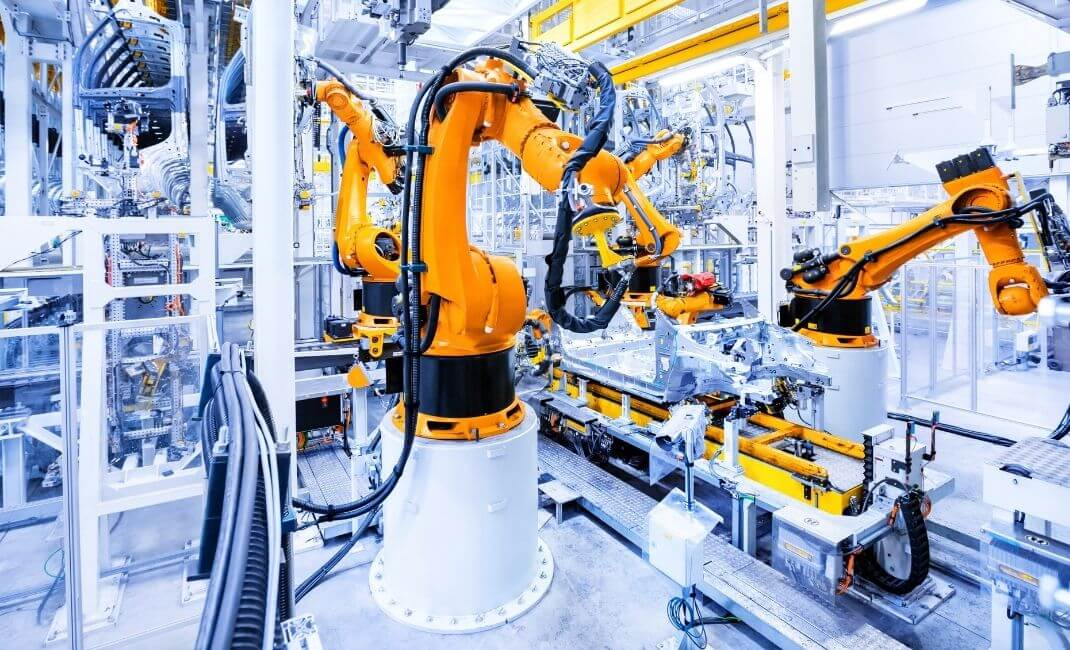
\includegraphics[width=13cm]{figs/automatizacion_industrial.jpg}
  \end{center}
  \caption{\centering Ejemplo de aplicación de automatización industrial.}
  \label{fig:automatizacion_industrial}
\end{figure}

La estructura de un sistema de automatización industrial se puede representar mediante un triángulo jerárquico de cinco niveles como se observa en la imagen ~\ref{fig:esquema_automatizacion}:

\begin{enumerate}
    \item \textbf{Nivel de gestión}: La alta gerencia usa sistemas ERP para controlar y monitorear todos los procesos de la empresa, desde la producción hasta ventas, compras y proyectos, asegurando eficiencia y alineación entre equipos.\cite{niveles_automatizacion_2}.
    \item \textbf{Nivel de operación}: Este nivel está controlado por el sistema MES. Un sistema MES conecta el mundo digital con la producción, permitiendo supervisar, sincronizar cada fase del proceso y monitorear la producción \cite{sistema_MES}. Este sistema integra datos de operaciones, mantenimiento, seguridad, logística y calidad, permitiendo a la gerencia tomar decisiones informadas sobre todo el proceso, desde las materias primas hasta el producto final. \cite{niveles_automatizacion_2}.
    \item \textbf{Nivel supervisor}: Compuesto por un ordenador industrial que utiliza software especializado para el control de procesos. Su principal objetivo es la parametrización y visualización del proceso y suele utilizars el protocolo de de comunicación Ethernet industrial \cite{niveles_automatizacion_1}.
    \item \textbf{Nivel de control}: Incluye dispositivos como PLCs que ejecutan las órdenes del nivel supervisor y controlan directamente la maquinaria en tiempo real. Estos pueden estar conectados a varios dispositivos de E/S y se comunican mediante protocolos industriales \cite{niveles_automatizacion_1}.
    \item \textbf{Nivel de campo}: Constituido por sensores y actuadores que interactúan directamente con el proceso físico conectados al PLC a través de un bus de campo. Los actuadores ejecutan acciones según las instrucciones recibidas normalmente a través de una conexión punto a punto con el PLC. \cite{niveles_automatizacion_1}. 
\end{enumerate}

Esta estructura permite una gestión eficiente y organizada de los procesos industriales, asegurando que cada componente funcione de manera integrada para optimizar la producción. 

\begin{figure} [h!]
  \begin{center}
    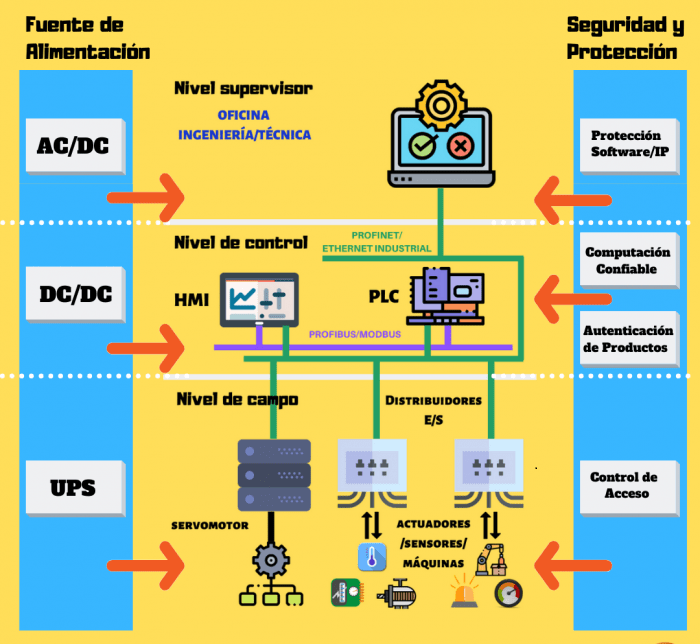
\includegraphics[width=15.5cm]{figs/esquema_automatizacion}
  \end{center}
  \caption{\centering Niveles de la pirámide de automatización. \cite{imagen_niveles_automatizacion}}  
  \label{fig:esquema_automatizacion}
\end{figure}  

\newpage

\subsection{Tipos de automatización industrial}

Los sistemas de automatización industrial se clasifican principalmente en cuatro tipos según su nivel de flexibilidad y aplicación en los procesos productivos:

\begin{enumerate}
    \item \textbf{Automatización fija}: Utilizada en procesos específicos y repetitivos donde no se requieren modificaciones en el diseño del producto debido a que aplicar modificaciones resulta casi imposible. Es ideal para la producción a gran escala de productos estables \cite{tipos_industrial}.
    \item \textbf{Automatización programable}: Aplicada en la fabricación por lotes, permite modificar el proceso mediante reprogramación, aunque esto puede consumir tiempo \cite{tipos_industrial}.
    \item \textbf{Automatización flexible}: Variante más avanzada de la automatización programable, que facilita cambios rápidos y automáticos en la producción sin interrupciones significativas \cite{tipos_industrial}.
    \newpage
    \item \textbf{Sistema Integrado de Automatización}: Conjunto de máquinas, procesos y datos sincronizados bajo un único sistema de control. Integra herramientas como CAD, CAM, robots y sistemas de transporte automatizados para optimizar la producción \cite{tipos_industrial}.
\end{enumerate}

\subsection{Ventajas y desventajas de la automatización industrial}

La automatización industrial ha transformado profundamente los procesos de producción, introduciendo tecnologías avanzadas que permiten aumentar la eficiencia, mejorar la calidad y reducir los costos operativos \cite{des_ventajas_1}. A continuación, se presentan las principales ventajas:

\begin{itemize}

 \item \textbf{Mayor productividad laboral}: La automatización acelera los procesos de producción, permitiendo fabricar más productos con una mejor calidad. Las nuevas tecnologías pueden operar de manera continua sin perder precisión, lo que incrementa la eficiencia y el rendimiento por hora de trabajo  \cite{des_ventajas_1}.

 \item \textbf{Mejora en la calidad del producto}: Uno de los principales beneficios de la automatización es la reducción de la cantidad de unidades defectuosas. Los sistemas automatizados garantizan una mayor uniformidad y precisión en la fabricación, cumpliendo con los estándares de calidad \cite{des_ventajas_2}.
   
\item \textbf{Reducción de costos de producción}: La automatización permite disminuir el gasto en mano de obra al reemplazar tareas repetitivas con maquinaria, lo que reduce el costo unitario de producción. Los sistemas automatizados operan de manera constante, aumentando la eficiencia y proporcionando un alto retorno de inversión al minimizar costos laborales, ausencias y otros gastos operativos \cite{des_ventajas_1}.

\item \textbf{Menos trabajo manual repetitivo}: En muchas industrias, es necesario supervisar constantemente variables como temperatura, presión o nivel de líquidos. Un sistema automatizado permite gestionar estas tareas mediante controladores de lazo cerrado, reduciendo la necesidad de intervención humana en actividades rutinarias \cite{des_ventajas_1}.

\item \textbf{Mayor seguridad}: Al implementar un sistema automatizado, los trabajadores pasan de realizar tareas directamente en el proceso a supervisarlas, lo que disminuye los riesgos laborales. Las máquinas pueden operar en entornos peligrosos o extremos, sustituyendo a los empleados en situaciones de alto riesgo, reduciendo así los accidentes laborales \cite{des_ventajas_2}.

\item \textbf{Facilita la monitorización remota}: Muchas operaciones industriales requieren ser controladas a distancia para una supervisión más eficiente. Los sistemas automatizados permiten la comunicación entre el área de producción y el centro de control, permitiendo a los operadores gestionar los procesos de manera remota \cite{des_ventajas_2}.

\end{itemize}

Sin embargo, junto con estos beneficios, como sucede en cualquier ámbito, también surgen desafíos y limitaciones que deben ser considerados por las empresas antes de implementar estos sistemas. Por eso, seguidamente se muestran algunas desventajas de la automatización industrial:

\begin{itemize}

\item \textbf{Aumento de la contaminación}: Muchas máquinas requieren motores que funcionan con combustibles o productos químicos que pueden generar emisiones contaminantes \cite{des_ventajas_1}.

\item \textbf{Menor flexibilidad}: Una máquina automatizada está diseñada para realizar tareas específicas, lo que limita la capacidad de adaptación a nuevas funciones en comparación con un trabajador humano. Actualmente, ciertas tareas, como el ensamblaje de productos con formas irregulares, siguen dependiendo del trabajo manual \cite{des_ventajas_1}.

\item \textbf{Altos costos de implementación}: La inversión inicial para adoptar un sistema automatizado es elevada. Además de los gastos en investigación y desarrollo, es necesario considerar los costos de mantenimiento, formación del personal y servicio técnico, lo que suma un desafío económico para las empresas que buscan automatizar sus procesos \cite{des_ventajas_2}.
\end{itemize}

\subsection{Equipos para la automatización industrial}

La automatización industrial se apoya en una amplia gama de dispositivos diseñados para controlar, supervisar y optimizar procesos dentro de entornos productivos. Entre estos equipos, destacan los Controladores Lógicos Programables (PLCs) y las Interfaces Hombre-Máquina (HMI), los cuales cumplen un papel fundamental en la implementación y operación de sistemas automatizados modernos.

\subsubsection{Controladores lógicos programables (PLCs)}

Un PLC (Controlador Lógico Programable) es una computadora diseñada específicamente para automatizar procesos industriales. Su tarea principal es controlar de manera eficiente y segura los sistemas que conforman una máquina o proceso, lo cual es clave para el avance tecnológico de las industrias. Estos dispositivos operan mediante un ciclo en el que se realiza un autodiagnóstico, se leen las entradas, se ejecuta el programa y finalmente se actualizan las salidas, lo que les permite adaptarse rápidamente a las condiciones cambiantes del entorno  \cite{plc_info}.

Existen distintos tipos de PLC, cada uno adaptado a las necesidades particulares de cada industria. Entre los más comunes se encuentran los modelos compactos, modulares o de banda estrecha. Marcas como Siemens y Allen Bradley son líderes en este mercado, ofreciendo una amplia variedad de productos y accesorios para mejorar la automatización de los procesos. Los PLCs se usan en una gran variedad de sectores, incluyendo la fabricación de cemento, plásticos, muebles, automotriz, transporte, energía y seguridad, ayudando a mejorar la eficiencia y reducir los costos operativos  \cite{plc_info}.

\begin{figure} [h!]
  \begin{center}
    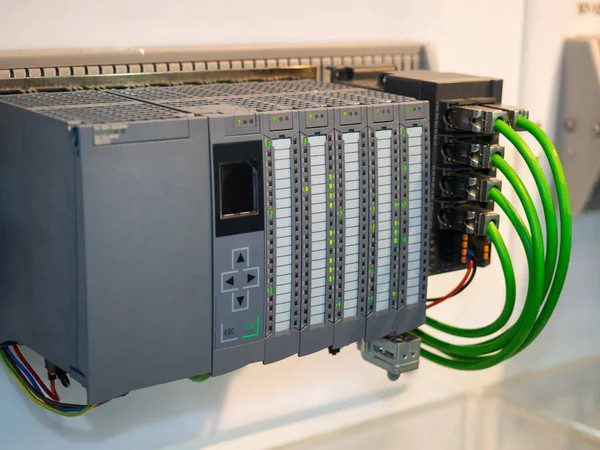
\includegraphics[width=9.5cm]{figs/info_plc}
  \end{center}
  \caption{\centering PLC de la serie Siemens S7-1500.}
  \label{fig:info_plc}
\end{figure} 

Una de las principales características de los PLC es su capacidad para controlar entradas y salidas de manera segura. Además, son compatibles con varios lenguajes de programación, lo que permite su fácil integración con sistemas de supervisión y control. Estos dispositivos pueden ser reprogramados según las necesidades del proceso, lo que les da gran flexibilidad y adaptabilidad en entornos industriales que están en constante cambio  \cite{plc_info}. \\

El lenguaje de programación utilizado para los PLCs y en este proyecto es el lenguaje KOP, también conocido como \textbf{Ladder}. Su popularidad se debe a su antigüedad, disponibilidad, mantenibilidad y facilidad de uso. Diseñado para imitar los diagramas eléctricos tradicionales, permite a técnicos e ingenieros familiarizados con estos esquemas adaptarse fácilmente a la programación en este lenguaje. Su naturaleza gráfica permite una comprensión rápida de la lógica del programa, lo que simplifica el proceso de mantenimiento y resolución de problemas \cite{ladder_info}.

\begin{figure} [h!]
  \begin{center}
    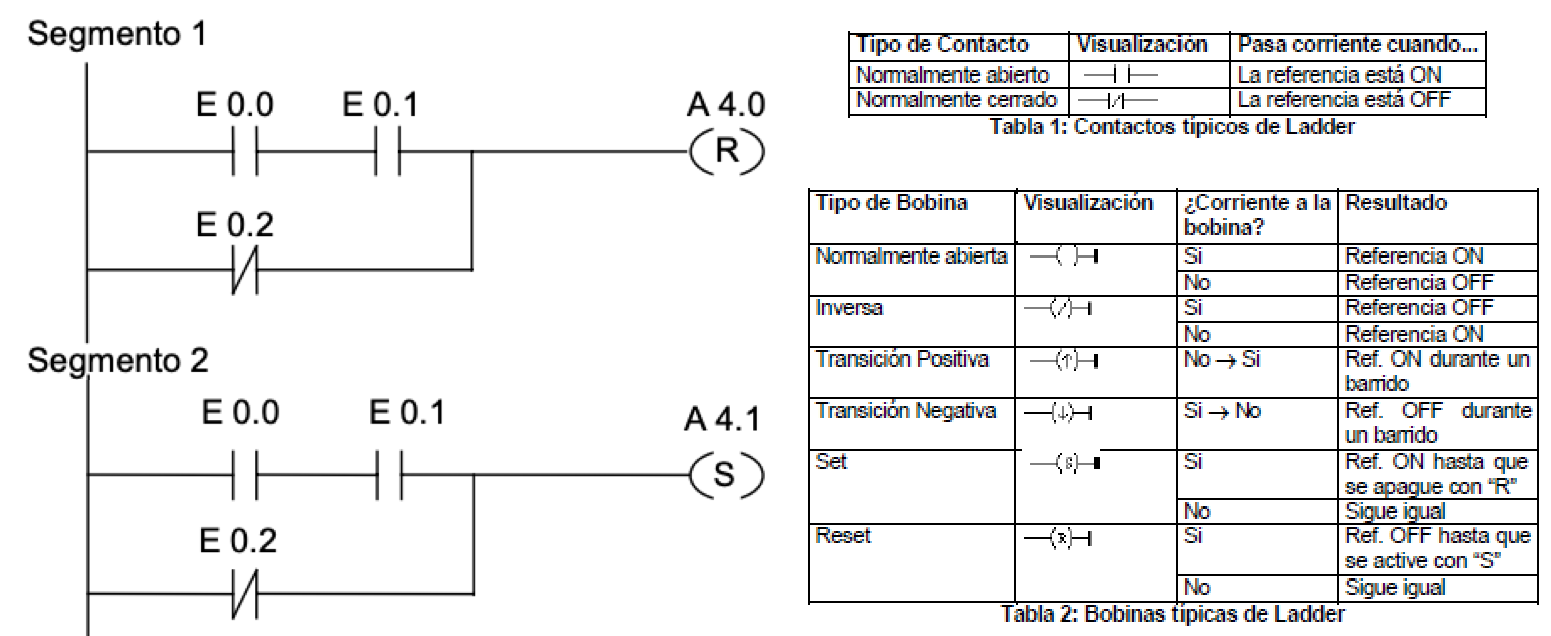
\includegraphics[width=15cm]{figs/ladder}
  \end{center}
  \caption{\centering Ejemplo del lenguaje de programación Ladder.}
  \label{fig:ladder}
\end{figure} 


\subsubsection{Interfaz humano máquina (HMI)}

Una Interfaz Hombre-Máquina (HMI) es un dispositivo que permite a los operarios comunicarse con sistemas automatizados dentro de un entorno industrial. Básicamente, actúa como una pantalla o panel táctil desde el cual se puede supervisar, controlar y ajustar el funcionamiento de una máquina o proceso. Los HMI permiten visualizar datos en tiempo real, como temperaturas, velocidades o estados de operación, y también enviar comandos para modificar parámetros o detener procesos si es necesario \cite{hmi}.

Además, estos dispositivos están pensados para funcionar en condiciones industriales exigentes, con diseños robustos y duraderos \cite{hmi}. También soportan múltiples idiomas y pueden adaptarse a distintos sectores y tipos de máquinas \cite{hmi}. En resumen, un HMI es una herramienta fundamental para mejorar la comunicación entre las personas y los sistemas automatizados, permitiendo un control más intuitivo, rápido y preciso de los procesos industriales.

\begin{figure} [h!]
  \begin{center}
    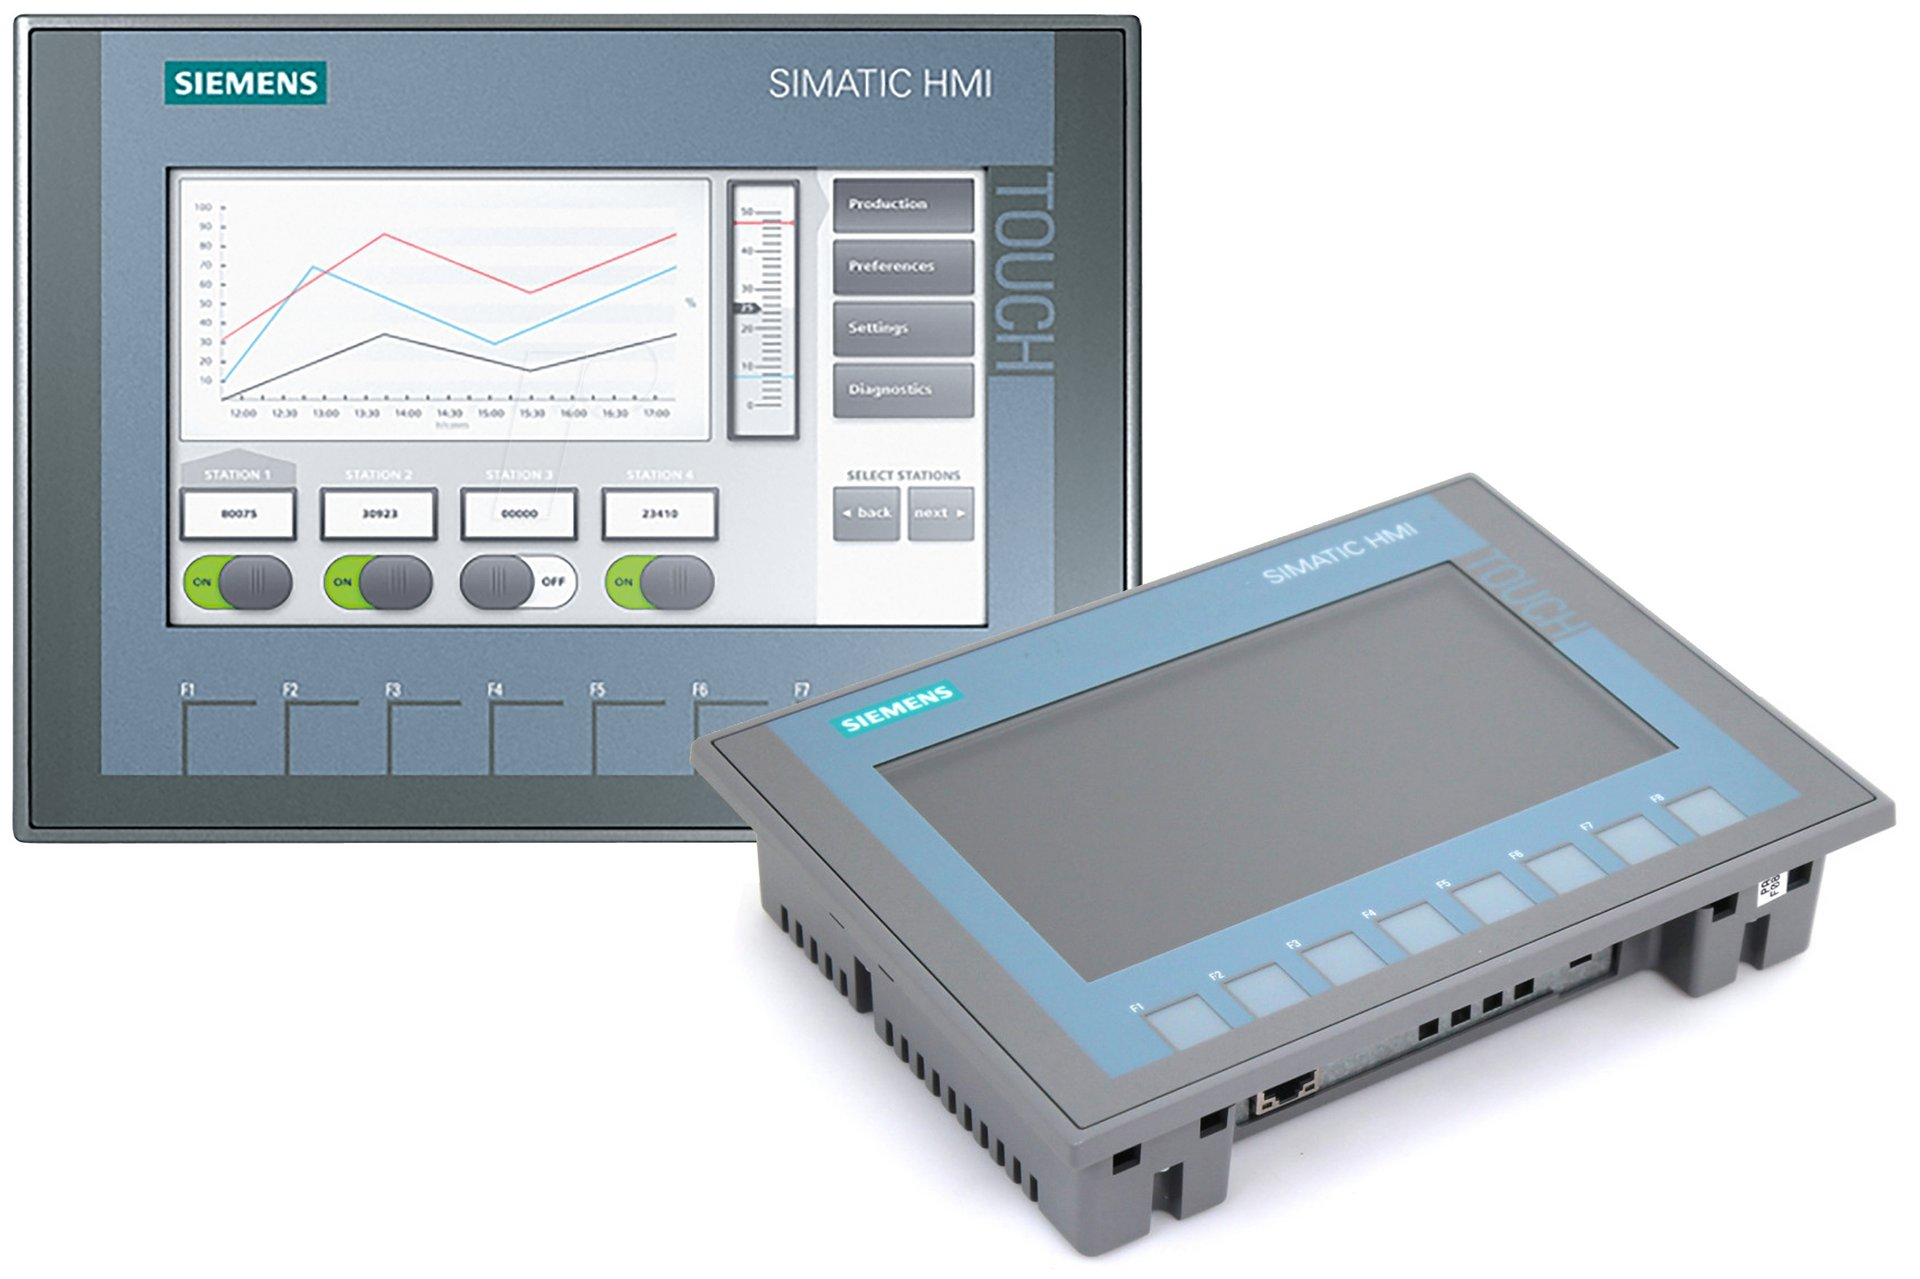
\includegraphics[width=13cm]{figs/HMI}
  \end{center}
  \caption{\centering HMI Siemens.}
  \label{fig:HMI}
\end{figure} 

\section{La robótica}
\label{sec:segundaseccion} % etiqueta para luego referenciar esta sección

La robótica es la disciplina científica que integra conocimientos de electrónica, mecánica e informática para desarrollar sistemas automatizados capaces de realizar tareas de manera autónoma o semiautónoma \cite{definicion_robot}. 

La robótica, en términos generales, abarca el diseño, construcción y programación de sistemas capaces de percibir su entorno, procesar información y ejecutar acciones de manera autónoma \cite{definicion_robot_2}. A diferencia de la robótica industrial, que se centra principalmente en tareas repetitivas, de alta precisión y en entornos estructurados como fábricas, la robótica tradicional se caracteriza por la diversidad de aplicaciones y la necesidad de adaptarse a contextos más variables y no estructurados. Esto implica la utilización de componentes versátiles, diseñados específicamente para cumplir funciones concretas en ámbitos como la robótica móvil, de exploración, educativa o de asistencia personal \cite{definicion_robot_2}.

En estos sistemas, los sensores juegan un papel crucial al proporcionar información del entorno que permite la adaptación del comportamiento del robot. Estos sensores, que pueden medir variables como luz, distancia, posición, velocidad, temperatura o fuerza, actúan como los "sentidos" del sistema robótico, y son fundamentales para su interacción efectiva con entornos complejos y no predecibles \cite{definicion_robot_2}. En contraste, en la robótica industrial los sensores suelen estar optimizados para tareas concretas dentro de procesos controlados y altamente repetitivos, donde las condiciones del entorno apenas varían.

Por su parte, el software y los algoritmos que controlan el comportamiento del robot en la robótica tradicional deben ser especialmente robustos, adaptativos y, en muchos casos, incorporar técnicas de inteligencia artificial o aprendizaje automático \cite{definicion_robot_2}. Esto permite al robot reaccionar de forma flexible a situaciones no previstas, algo menos común en la robótica industrial, donde los algoritmos suelen estar más orientados a la eficiencia, estabilidad y cumplimiento exacto de ciclos de producción \cite{definicion_robot_2}. Finalmente, los actuadores son los responsables de ejecutar las decisiones del sistema de control y deben estar diseñados para responder con precisión y versatilidad, siendo capaces de adaptarse a tareas muy variadas, a diferencia de los actuadores industriales, que suelen estar optimizados para movimientos repetitivos y bien definidos en líneas de montaje automatizadas \cite{definicion_robot_2}.

\begin{figure} [h!]
  \begin{center}
    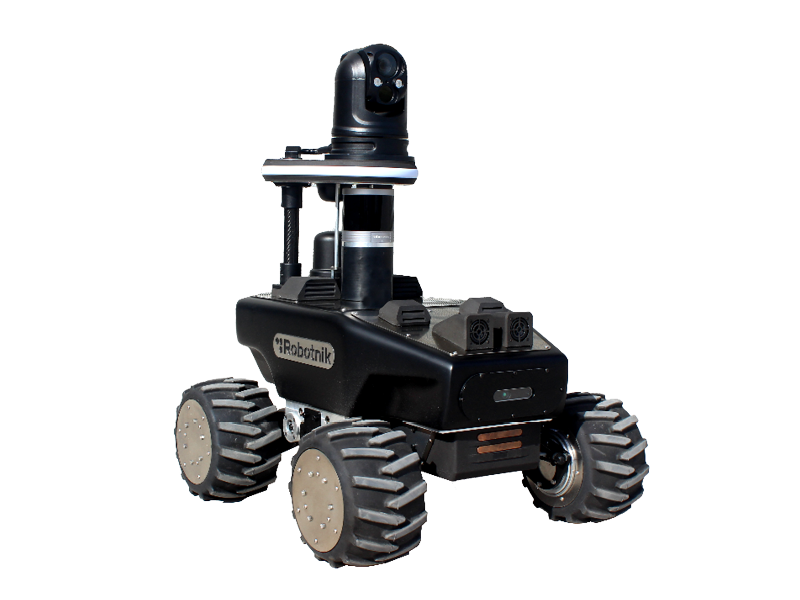
\includegraphics[width=8cm]{figs/Robot_intro}
  \end{center}
  \caption{\centering RB-WATCHER de Robotink.}
  \label{fig:Robot_intro}
\end{figure}

\subsection{Robótica industrial}

Según la norma internacional ISO 8373:2021 un robot industrial se define como ``un manipulador multifuncional, reprogramable y controlado automáticamente, programable en tres o más ejes que puede estar fijo en un área o móvil para su uso en aplicaciones de automatización industrial'' \cite{definicion_iso}. Todo ello a partir de trayectorias variables para ejecutar diversas tareas cíclicas y adaptables. 

La robótica industrial es una disciplina de la ingeniería robótica dedicada al diseño, desarrollo y fabricación de robots industriales con el propósito de automatizar tareas repetitivas tradicionalmente realizadas por seres humanos. Estos sistemas robóticos se caracterizan por seguir una secuencia de instrucciones predefinidas, ejecutando ciclos de trabajo continuos en líneas de producción de diversos sectores industriales. Estos robots son considerados industriales debido a que se utilizan en la industria manufacturera en sectores como la automoción, electrónica, alimentación, farmacéutico... En ellos contribuyen significativamente a mejorar la eficiencia, la velocidad y la calidad de los procesos productivos \cite{info_robotica_industrial_1}. 

A diferencia de los robots de servicio, los robots industriales operan en entornos altamente controlados, lo que simplifica su programación y control. Debido a estas condiciones estables, estos robots suelen tener más de tres grados de libertad, permitiéndoles realizar movimientos complejos con gran precisión. Aunque su aplicación principal ha sido históricamente en entornos industriales, su uso se ha expandido hacia sectores como la minería, la agricultura, el comercio y la salud, demostrando su versatilidad y adaptabilidad. \\

\begin{figure} [h!]
  \begin{center}
    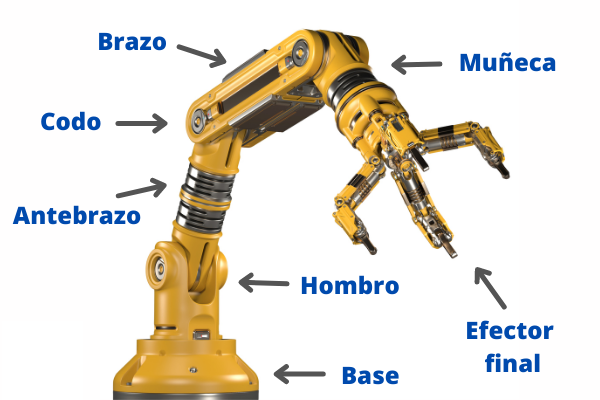
\includegraphics[width=9cm]{figs/brazo_industrial}
  \end{center}
  \caption{\centering Partes de un brazo robótico industrial.}
  \label{fig:brazo_industrials}
\end{figure}

Para que un brazo robótico sea considerado industrial, debe cumplir con una serie de características técnicas y funcionales que lo hagan adecuado para entornos de producción. Entre ellas, destacan la precisión y la repetibilidad, que permiten realizar tareas con tolerancias muy ajustadas. También debe tener una estructura robusta y una capacidad de carga suficiente según la aplicación, así como al menos seis grados de libertad para poder ejecutar movimientos complejos \cite{brazo_industrial}.

Otra característica fundamental es la velocidad de operación, ya que en entornos industriales es clave mantener ritmos de trabajo altos. Además, debe ser fácilmente programable y compatible con sistemas de automatización como PLCs o entornos como ROS, y permitir la integración con sensores, cámaras o herramientas específicas  \cite{brazo_industrial}.

Desde el punto de vista de seguridad y conectividad, debe cumplir con normativas como la ISO 10218 y ser compatible con protocolos industriales como PROFINET o EtherCAT \cite{brazo_industrial}. 

Desde la aparición de los primeros prototipos de robots industriales, ha surgido un debate sobre su impacto en el empleo humano, con preocupaciones respecto a una posible sustitución de la mano de obra. Sin embargo, numerosos estudios sostienen que, lejos de desplazar a los trabajadores, estos sistemas robóticos buscan mejorar las condiciones laborales, eliminando tareas monótonas o peligrosas \cite{info_robotica_industrial_2}. 

\section{Unión entre la automatización y la robótica}
\label{sec:terceraseccion}

Entrando al siglo XXI se desarrollan los primeros robots colaborativos, conocidos como cobots, concebidos para cooperar de manera directa con las personas. Estos dispositivos se caracterizan por su seguridad, adaptabilidad y facilidad de programación, convirtiéndose en una solución ideal para entornos industriales donde es necesario combinar tareas manuales y automatizadas  \cite{intro_union}. 

En los años 2010, la Industria 4.0 emergió como una nueva fase en la manufactura, caracterizada por la digitalización y la interconexión de sistemas de producción.  Los robots industriales se convirtieron en componentes clave de las fábricas inteligentes, colaborando estrechamente con humanos y otros sistemas automatizados para optimizar la eficiencia y la flexibilidad en la producción \cite{intro_union}. 

\subsection{Comunicaciones entre los dispositivos}

Las comunicaciones entre dispositivos industriales son fundamentales para que los procesos de producción actuales funcionen de forma segura, eficiente y automatizada \cite{intro_com}. Gracias a ellas, sensores, actuadores, controladores y sistemas de gestión pueden intercambiar datos constantemente, asegurando que todo el proceso esté coordinado y optimizado. El objetivo principal de estas comunicaciones es transformar la información captada del entorno en datos útiles que faciliten la toma de decisiones rápidas y eficaces \cite{intro_com}. Esto no solo mejora la eficiencia de la producción, sino que también ayuda a prevenir errores, optimizar el uso de recursos y mantener los procesos en marcha sin interrupciones. A diferencia de las redes convencionales, las comunicaciones industriales deben cumplir con requisitos muy exigentes: alta fiabilidad, resistencia a condiciones adversas, capacidad para operar en tiempo real y determinismo. \cite{intro_com}. 

La tecnología de \textbf{bus de campo} apareció a finales de los años 80 con el objetivo de ofrecer un método estandarizado para conectar múltiples dispositivos de campo en entornos industriales. El bus de campo es una red de comunicación industrial bidireccional y multipunto que conecta dispositivos de campo inteligentes, sustituyendo los sistemas de control centralizados por redes distribuidas \cite{info_bus}. Existen múltiples variantes desarrolladas por fabricantes para diferentes nichos destacando: PROFIBUS en automoción y control de procesos, CANbus en el sector automotriz y maquinaria y Foundation Fieldbus en industrias de petróleo y gas entre otros \cite{bus_vs_ethernet}.

\begin{figure} [h!]
  \begin{center}
    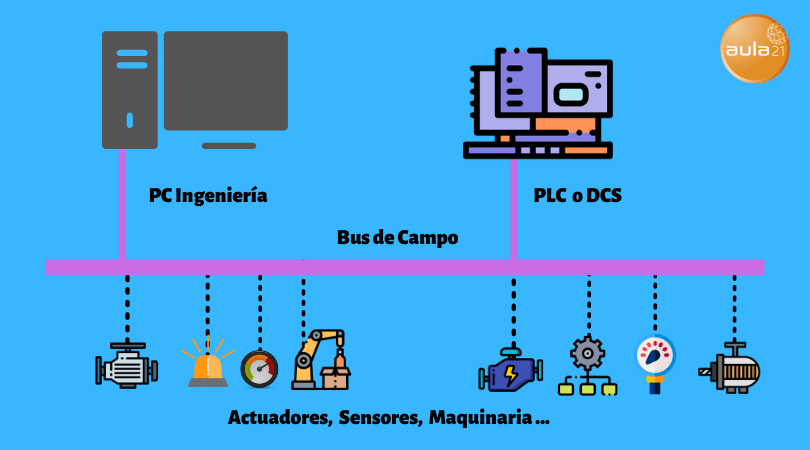
\includegraphics[width=15cm]{figs/bus_de_campo}
  \end{center}
  \caption{\centering Ejemplo básico de dus de campo. \cite{info_bus}}
  \label{fig:bus_de_campo}
\end{figure} 

Por otro lado, la tecnología \textbf{Ethernet industrial} surge como una evolución de Ethernet tradicional, adaptándose a los estrictos requerimientos de entornos industriales donde la robustez, el intercambio de datos en tiempo real y la resistencia a interferencias son esenciales. A partir del estándar IEEE 802.3, Ethernet industrial integra mejoras específicas para la automatización, soportando protocolos como Modbus TCP/IP, PROFINET y EtherCAT \cite{bus_vs_ethernet}.

Entre sus principales ventajas frente a los sistemas de bus de campo tradicionales destacan sus altas velocidades de comunicación (desde 10 Mbps hasta 10 Gbps), su apertura e interoperabilidad, la escalabilidad de la red y su rentabilidad. Estas características permiten su uso tanto en el monitoreo en tiempo real como en la integración de sistemas de gestión y supervisión de plantas industriales, convirtiéndolo en la base de las redes industriales modernas \cite{bus_vs_ethernet}.

\begin{figure} [h!]
  \begin{center}
    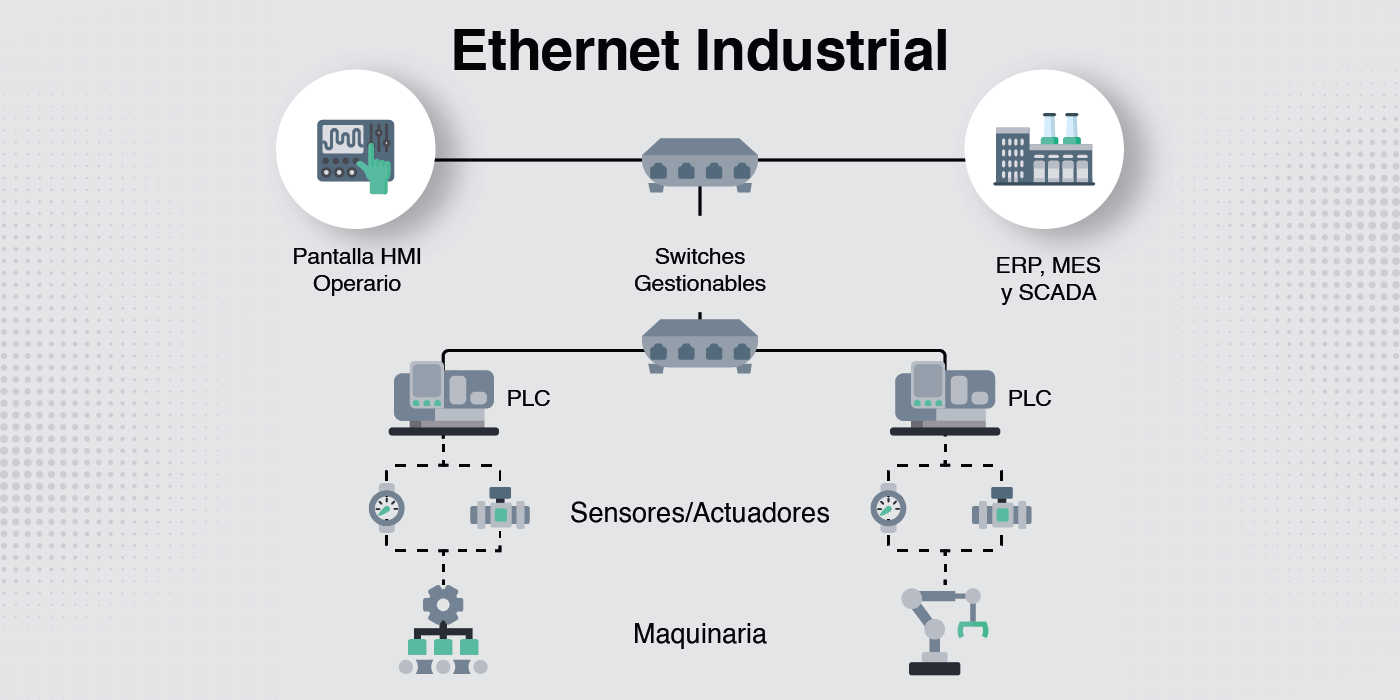
\includegraphics[width=15.5cm]{figs/ethernet_industrial}
  \end{center}
  \caption{\centering Ejemplo básico de red de ethernet industrial. \cite{ethernet_imagen}}
  \label{fig:ethernet_industrial}
\end{figure} 


\subsection{Metodología de la automatización industrial}

En la automatización industrial, es fundamental seguir una metodología clara que permita diseñar, implementar y controlar los procesos de forma ordenada y eficiente. Para ello, existen herramientas y enfoques que ayudan a representar el comportamiento del sistema, identificar sus distintos modos de funcionamiento y supervisar su estado en tiempo real.

Una de las herramientas más utilizadas es el GRAFCET, un lenguaje gráfico que permite describir de forma sencilla el funcionamiento secuencial de un sistema. Junto a él, la guía GEMMA ayuda a identificar los distintos modos de operación del sistema (como arranque, parada o fallo), y sirve como complemento al GRAFCET para organizar mejor el control general del proceso. Por último, los sistemas SCADA juegan un papel clave en la supervisión de procesos industriales, permitendo al operador visualizar en tiempo real lo que ocurre en planta, modificar parámetros y detectar posibles errores de forma rápida.

\newpage

\subsubsection{GRAFCET}

El modelo GRAFCET (Graphe Fonctionnel de Commande Étape Transition) es un método gráfico que se utiliza en la automatización industrial para representar y controlar procesos secuenciales. Creado en 1977 por la AFCET (Asociación Francesa para la Cibernética Económica y Técnica), su objetivo es describir el comportamiento de los sistemas de control mediante un diagrama de etapas y transiciones \cite{grafcet_info}. Esto no es un lenguaje de programación, sino una forma de resolver el problema de automatización secuencial previo a su programación en el PLC. A continuación, se describen los distintos elementos que conforman un GRAFCET:

\begin{enumerate}
    \item \textbf{Etapas}: Se representan como cuadros numerados en el diagrama. Cada etapa indica un estado específico del sistema y las acciones que deben llevarse a cabo cuando esa etapa está activa. La etapa inicial se representa con un doble cuadrado.
    \item \textbf{Transiciones}: Son las condiciones que deben cumplirse para que el sistema pase de una etapa a otra. Estas condiciones se representan por líneas que cruzan de manera perpendicular las etapas. Las transiciones se activan cuando se cumple una condición lógica, como el final de un proceso o la llegada de una señal.
    \item \textbf{Uniones}: Representan las conexiones entre varias etapas y permiten que se ejecuten acciones simultáneas en diferentes partes del sistema. Las uniones facilitan la ejecución de procesos en paralelo.
    \item \textbf{Acciones}: Son las operaciones que se realizan cuando una etapa está activa. Estas acciones están directamente vinculadas a la etapa correspondiente.
\end{enumerate}
    
Este modelo resulta muy útil en procesos industriales donde las operaciones siguen una secuencia lógica y estructurada. Se utiliza comúnmente en la programación de PLCs (Controladores Lógicos Programables), ya que permite controlar sistemas paso a paso y asegura que las acciones se realicen de manera secuencial \cite{grafcet_info}.

\begin{figure} [h!]
  \begin{center}
    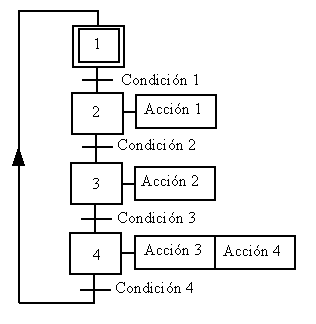
\includegraphics[width=8cm]{figs/grafcet_def}
  \end{center}
  \caption{\centering Ejemplo básico de GRAFCET.}
  \label{fig:grafcet_def}
\end{figure} 

Una vez creado el Grafcet, para poder introducir la lógica pensada en el PLC, hay que traducir la información al lenguaje ladder, que es el cual entiende el PLC. Para ello se deben asignar direcciones de memoria en el PLC a cada etapa, entradas, salidas y demás elementos como contadores o temporizadores. Una vez traducido el Grafcet al lenguaje Ladder e introducido en el PLC ya se puede ejecutar la secuencia realizada del sistema.

\subsubsection{Guia GEMMA}

La Guía GEMMA (Guía para la Elaboración de los Modelos de los Modos de Marcha y Parada de una Automatización) es una metodología utilizada en el ámbito de la automatización industrial para representar de forma clara y estructurada los diferentes modos de funcionamiento de una máquina o sistema  \cite{guia_gemma}. La guía GEMMA está compuesta por bloques que representan cada uno de estos modos y sus posibles transiciones, lo que proporciona una visión global y ordenada del comportamiento del sistema  \cite{guia_gemma}.

El núcleo de la guía se basa en tres grandes categorías: funcionamiento, parada o puesta en marcha, y defecto. En cada categoría se pueden identificar varios subestados como:

\begin{itemize}
  \item  \textbf{Funcionamiento}: La producción en curso o marcha de cierre \cite{guia_gemma}.
  \item \textbf{Parada o puesta en marcha}: La parada al estado inicial o de final de ciclo \cite{guia_gemma}.
  \item \textbf{Defecto}: La parada de emergencia \cite{guia_gemma}. 
\end{itemize} 

Además de su valor como herramienta de planificación, GEMMA se integra fácilmente con otras metodologías como el GRAFCET, permitiendo diseñar automatismos más seguros y eficientes. Al normalizar los distintos modos de operación y facilitar la interpretación de los estados de una automatización, la Guía GEMMA se ha convertido en un recurso esencial para la automatización de procesos.

\begin{figure} [h!]
  \begin{center}
    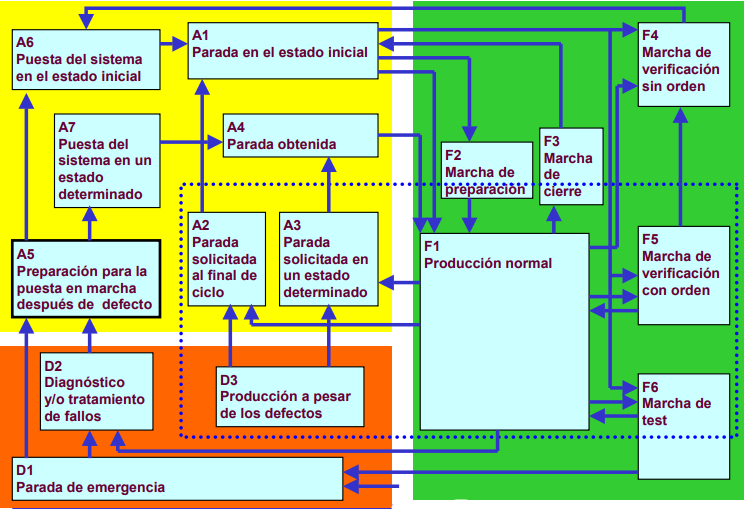
\includegraphics[width=15cm]{figs/guia_gemma}
  \end{center}
  \caption{\centering Ejemplo de guía gemma complejo. \cite{guia_gemma}}
  \label{fig:guia_gemma}
\end{figure} 

\subsubsection{Sistemas SCADA}

Un sistema SCADA (Supervisory Control and Data Acquisition) es una herramienta clave en la automatización industrial, diseñada para supervisar y controlar procesos a distancia mediante la recopilación y análisis de datos en tiempo real \cite{scada}. Estos sistemas permiten monitorear variables críticas como temperatura, presión o caudal, facilitando una operación eficiente y segura de plantas industriales, líneas de producción, redes eléctricas o infraestructuras inteligentes \cite{scada}.

Los sistemas SCADA recopilan información a través de sensores y dispositivos conectados a una red de comunicaciones, ya sea cableada o inalámbrica. Esta información se procesa en un software especializado que permite visualizar los datos, generar alarmas ante anomalías y controlar equipos de forma remota \cite{scada}. Entre sus funciones principales se incluyen la monitorización en tiempo real, análisis de datos, generación de alertas y control de dispositivos como válvulas o motores \cite{scada}.

\begin{figure} [h!]
  \begin{center}
    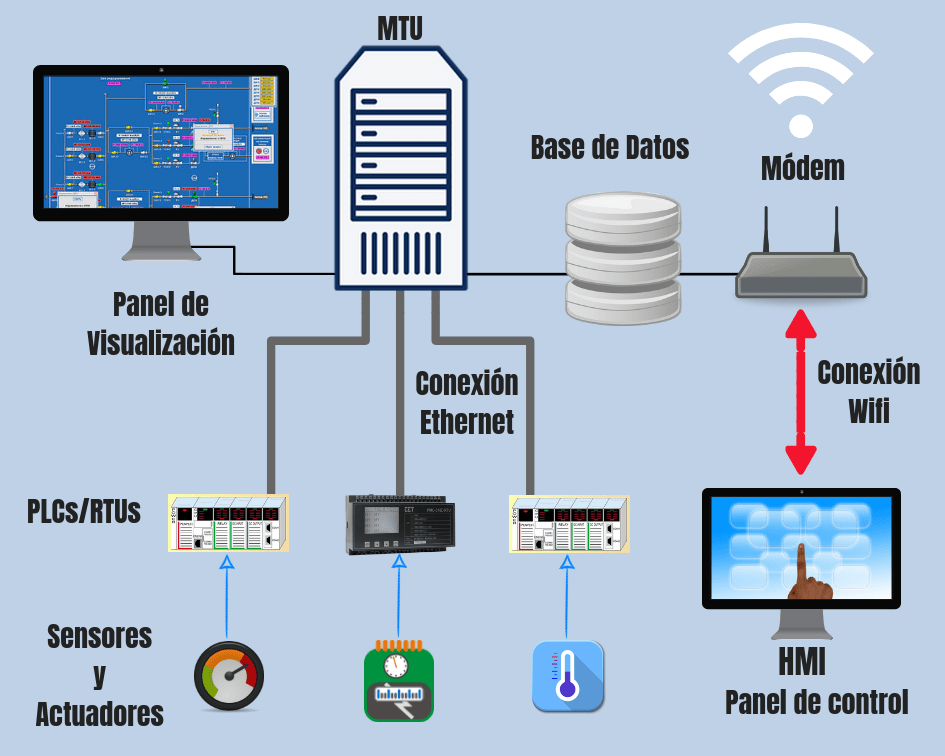
\includegraphics[width=15cm]{figs/SCADA}
  \end{center}
  \caption{\centering Ejemplo de un diagrama básico con sistema SCADA. \cite{scada_img}}
  \label{fig:SCADA}
\end{figure} 

Existen diferentes tipos de sistemas SCADA según su arquitectura: centralizados, donde todos los componentes están en una misma ubicación; distribuidos, con componentes separados conectados por una red; y híbridos, que combinan características de ambos \cite{scada}. Implementar un sistema SCADA adecuado puede mejorar significativamente la eficiencia operativa y la capacidad de respuesta ante incidencias en entornos industriales.

\section{Motivación del trabajo}
\label{sec:cuartaseccion}

La automatización industrial representa una opción laboral muy atractiva, con la transformación digital impulsada por la Industria 4.0 y el auge de tecnologías como el Internet de las Cosas (IoT), la robótica o la inteligencia artificial, la demanda de profesionales cualificados en este ámbito no ha dejado de crecer. Sectores como la automoción, la alimentación o la logística están apostando cada vez más por la automatización para mantenerse competitivos en un mercado globalizado.

\newpage

\begin{figure} [h!]
  \begin{center}
    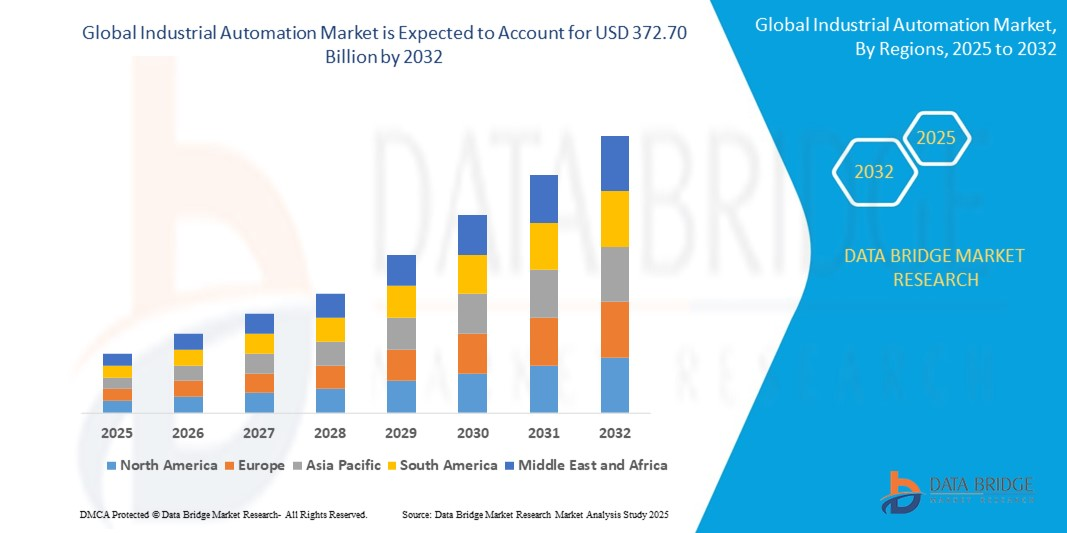
\includegraphics[width=15cm]{figs/grafico_futuro}
  \end{center}
  \caption{\centering Tendencias del mercado global de automatización industrial. \cite{grafico_empleabilidad}}
  \label{fig:grafico_futuro}
\end{figure} 

Como se observa en la figura  ~\ref{fig:grafico_futuro}, se preveé que cada año se invierta más dinero en la automatización industrial,
por lo que este campo tiene un gran futuro. La producción industrial en masa seguirá siendo clave para satisfacer la demanda del mercado, impulsada por el crecimiento demográfico y el alto nivel de consumo. Por otro lado, el desarrollo continuo de nuevas tecnologías y robots hace que el sector esté en constante evolución, tal y como viene ocurriendo desde sus orígenes en la década de 1940.

La creciente escasez de perfiles especializados en el ámbito de la automatización y la robótica incrementa notablemente las oportunidades laborales para quienes cuentan con formación en estas áreas. La familiaridad con simuladores durante la etapa académica puede representar un valor añadido en los procesos de selección, al proporcionar una ventaja comparativa frente a candidatos sin experiencia práctica con sistemas físicos. A ello se suma la existencia de salarios de entrada competitivos, que tienden a incrementarse con la experiencia y que, en general, permiten acceder a una buena calidad de vida.

El trabajo tiene como objetivo el desarrollo de una aplicación basada en el uso de dos simuladores didácticos, concebida como una herramienta de apoyo para facilitar el aprendizaje de contenidos relacionados con la robótica y la automatización. La utilización de este tipo de recursos permite fomentar un aprendizaje más interactivo y dinámico, lo cual contribuye a una mayor motivación del alumnado y a una mejor asimilación de los conceptos teóricos. Asimismo, la combinación de entornos virtuales con prácticas reales constituye una estrategia eficaz para reforzar la formación técnica y preparar al estudiante para los desafíos propios del ámbito profesional.

A lo largo de la formación académica de los ingenieros, se adquieren conocimientos en diferentes disciplinas, tanto desde el punto de vista teórico como práctico. Una característica común en numerosas asignaturas es la utilización de simuladores, los cuales permiten aplicar los conocimientos adquiridos en entornos virtuales controlados. Estos entornos ofrecen múltiples ventajas, entre las que se incluyen la posibilidad de programar sin riesgo de dañar un robot físico, la personalización del entorno de trabajo en función de la aplicación deseada, y la experimentación con distintas configuraciones de forma sencilla y sin incurrir en costes adicionales.

Aun así, trabajar solo con simuladores no es lo mismo que hacerlo con sistemas reales. La experiencia práctica que se obtiene al enfrentarse a un entorno físico es mucho más rica y completa. En la realidad, hay que lidiar con errores de sensores, fallos en los actuadores, problemas mecánicos o situaciones imprevistas que obligan a pensar y reaccionar. Estas experiencias ayudan a desarrollar habilidades muy valiosas, como la capacidad de resolver problemas, tomar decisiones rápidas y adaptarse a los cambios, cosas que un simulador, por muy avanzado que sea, no siempre puede ofrecer.
